\subsection{Car model}

The car model consists of two sub-models: the wheel model and the body model.
The wheel model is just a slightly modified cylinder.

The main difficulty in modeling the car's body is getting the proportions right.
Otherwise, the model looks very unnatural.
After some unsuccessful attempts to create the model free-hand, we decided to use blueprints of an existing car (1965 Ford Mustang) for modeling.
The process of modeling the car based on blueprints (side view) is depicted in \autoref{fig:mustang-blender}.

\begin{figure}[h]
    \centering
    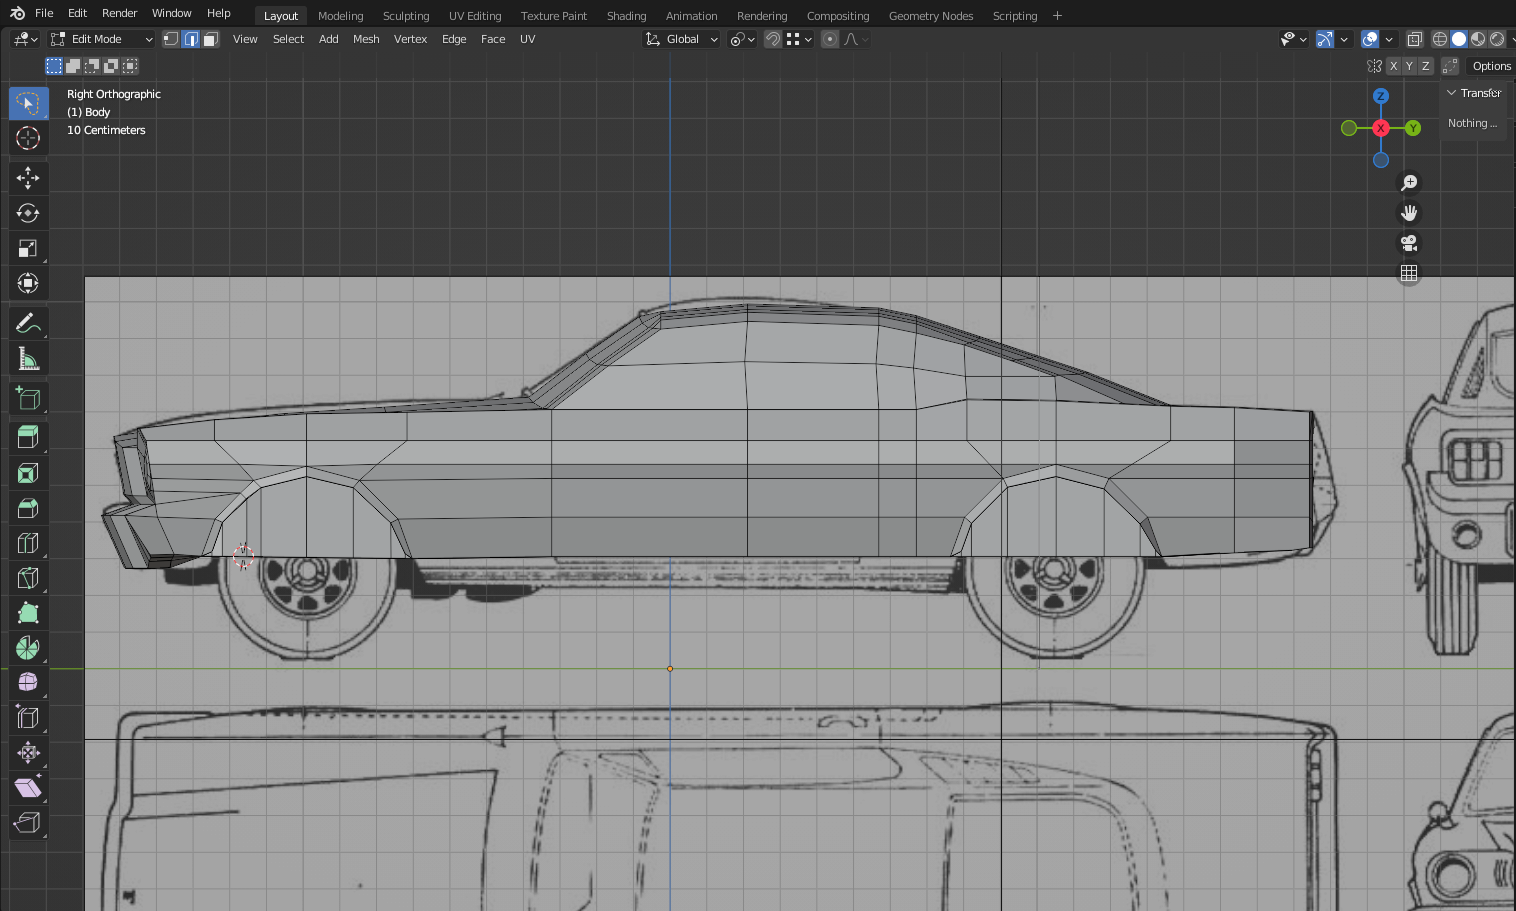
\includegraphics[width=0.8\textwidth]{chapters/theoretical_foundations/sections/models/resources/mustang-blender.png}
    \caption{Modeling in Blender based on blueprints}
    \label{fig:mustang-blender}
\end{figure}
